\documentclass{article}

\usepackage{graphicx}
\usepackage{tikz}
\usepackage{tikzsymbols}
\usetikzlibrary{calc,patterns,shapes.geometric}
\pagestyle{empty}
\usepackage[margin=0pt]{geometry}
\geometry{papersize={14in,12in}}

\def\centerarc[#1](#2)(#3:#4:#5){\draw[#1] ($(#2)+({#5*cos(#3)},{#5*sin(#3)})$) arc (#3:#4:#5);}

\begin{document}
	\begin{figure}
		\centering
		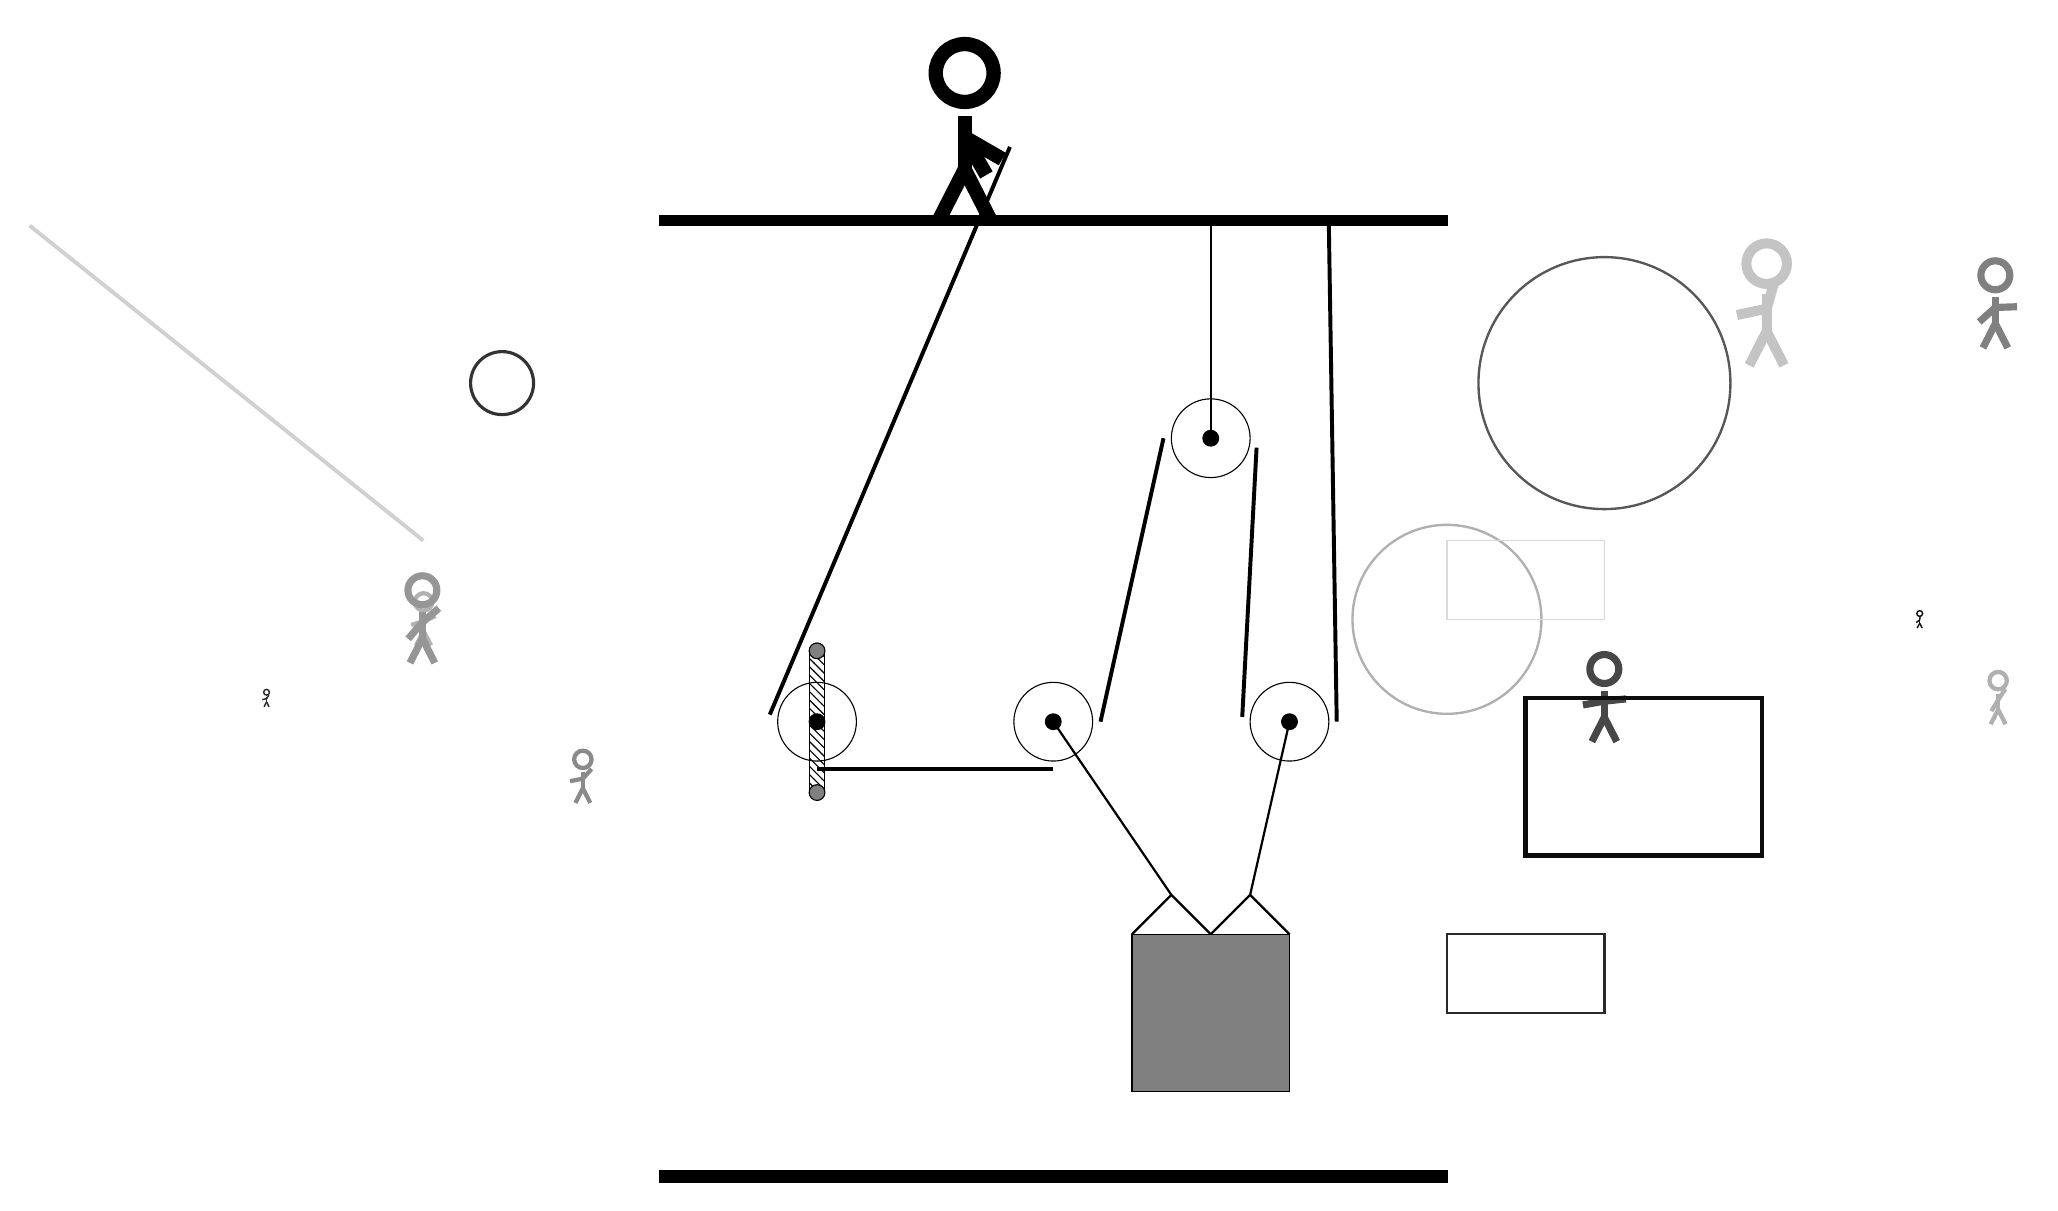
\begin{tikzpicture}
			%%%%% START %%%%%
			
			\draw[fill=black] (-4, 9) rectangle (6, 9.125);
			
			\draw (1, 2.7) circle (0.5);
			\draw[fill=black] (1, 2.7) circle (0.1);
			
			\draw (3, 6.3) circle (0.5);
			\draw[fill=black] (3, 6.3) circle (0.1);
			\draw[thick] (3, 6.3) -- (3, 9);
			
			\draw (4, 2.7) circle (0.5);
			\draw[fill=black] (4, 2.7) circle (0.1);
			
			\draw[thick] (4, 2.7) -- (3.5, 0.5);
			\draw[thick] (1, 2.7) -- (2.5, 0.5);
			\draw[thick]  (2, 0) -- (2.5, 0.5) -- (3, 0);
			\draw[thick]  (3, 0) -- (3.5, 0.5) -- (4, 0);
			\draw[fill=black!50] (2, 0) rectangle (4, -2);
			
			\node[line width=0.3mm, color=black!30] at (-7, 4) {\Strichmaxerl[3][17][23]};
			
			\node[line width=0.3mm, color=black!41] at (-7, 4) {\Strichmaxerl[5][49][41]};
			\draw [line width=0.3mm, color=black!66](8, 7) circle (1.6);
			\node[line width=0.5mm, color=black!31] at (13, 3) {\Strichmaxerl[3][59][57]};
			
			\draw[line width=0.3mm, color=black!84] (8, -1) rectangle (6, 0);
			\node[line width=0.4mm, color=black!83] at (-9, 3) {\Strichmaxerl[1][12][58]};
			
			\draw [line width=0.4mm, color=black!80](-6, 7) circle (0.4);
			\node[line width=0.5mm, color=black!50] at (13, 8) {\Strichmaxerl[5][42][2]};
			\node[line width=0.4mm, color=black!46] at (-5, 2) {\Strichmaxerl[3][11][48]};
			
			\draw [line width=0.3mm, color=black!31](6, 4) circle (1.2);
			
			\node[line width=0.6mm, color=black!23] at (10, 8) {\Strichmaxerl[7][12][74]};
			
			\node[line width=0.3mm, color=black!72] at (8, 3) {\Strichmaxerl[5][10][6]};
			\draw[line width=0.5mm, color=black!18](-7, 5) -- (-12, 9);
			
			\node[line width=0.5mm, color=black!93] at (12, 4) {\Strichmaxerl[1][36][83]};
			\draw[line width=0.6mm, color=black!95] (7, 1) rectangle (10, 3);
			\draw[line width=0.2mm, color=black!14] (8, 5) rectangle (6, 4);
			
			
			\draw (-2, 2.7) circle (0.5);
			\draw[fill=black] (-2, 2.7) circle (0.1);
			\draw[pattern=north west lines, pattern color=black] (-2.1, 3.6) rectangle (-1.9, 1.8);
			\draw[fill=black!50] (-2, 3.6) circle (0.1);
			\draw[fill=black!50] (-2, 1.8) circle (0.1);
			
			\draw[line width=0.5mm] (0.45, 10) -- (-2.6, 2.79);
			\centerarc[line width=0.5mm](-2, 2.7)(160:270:0.6);
			\draw[line width=0.5mm](-2, 2.1) -- (1, 2.1);
			\centerarc[line width=0.5mm](1, 2.7)(270:360:0.6);
			\draw[line width=0.5mm] (1.6, 2.7) -- (2.4, 6.3);
			\centerarc[line width=0.5mm](3, 6.3)(-20:180:0.6);
			\draw[line width=0.5mm](3.582, 6.18) -- (3.4, 2.76);
			\centerarc[line width=0.5mm](4, 2.7)(160:360:0.6);
			\draw[line width=0.5mm](4.6, 2.7) -- (4.5, 9);
			
			\node at (-0.07, 10.2) {\Strichmaxerl[10][120][-30]};
			
			\draw[fill=black] (-4, -3) rectangle (6, -3.15);
			
			%%%%% END %%%%%
		\end{tikzpicture}
	\end{figure}	
\end{document}